\documentclass{article}
\usepackage{iclr2026_conference,times}
\input{math_commands.tex}
\usepackage{hyperref}
\usepackage{url}
\usepackage{booktabs}
\usepackage{graphicx}
\usepackage{amsmath}
\usepackage{amssymb}
\usepackage{xcolor}
\usepackage{multirow}
\usepackage{xspace}
\usepackage{algorithm}
\usepackage{algpseudocode}

\title{How Far Can Pure Geometry Go? \\ A Systematic Boundary Analysis of Training-Free \\ LiDAR Instance Segmentation}

\author{Anonymous Authors}

\newcommand{\sepsam}{SepSAM\xspace}
\newcommand{\method}{\sepsam}

\begin{document}
\maketitle

\begin{abstract}
We present the first systematic quantification of the capability boundary for
zero-training, pure-geometric LiDAR instance segmentation. The core challenge is that
point cloud geometry alone carries limited semantic signal: across 209K fragments and
15K SAM masks, no geometric descriptor exceeds AUC 0.7 for distinguishing objects from
background. We bridge SAM to pure LiDAR via DBSCAN over-segmentation and skeleton-based
geometric prompt sampling---requiring no training data, human annotations, or RGB
imagery. Through six independently tested and empirically disconfirmed improvement
hypotheses on SemanticKITTI (4,071 frames), we establish a tightening ceiling chain:
DBSCAN oracle at 39.4\% mIoU, pipeline bound $\leq$35\%, and empirical result of
31.6\%. Class-agnostic evaluation closes the loop: removing semantic class labels
changes mIoU by only 0.3 percentage points (29.9\% vs.\ 30.2\%), confirming
that geometric matching quality, not semantic confusion, is the bottleneck. Our core finding is a hard
ceiling of $\sim$30\% mIoU for zero-training pure-geometric LiDAR instance
segmentation---demonstrating that semantic information is fundamentally irreplaceable
and providing a quantified calibration point for the field.
\end{abstract}

% ============================================================
\section{Introduction}
% ============================================================

LiDAR instance segmentation is a cornerstone of autonomous driving perception.
State-of-the-art approaches---whether point-based, voxel-based, or
range-view-based---share a common dependency: they require large-scale
human-annotated semantic labels, co-located RGB imagery, or
both~\cite{dusi2025lidar}. These annotations are expensive to acquire,
domain-specific, and brittle under sensor or environment shifts. A natural
question arises: if we strip away all semantic information and RGB input,
retaining only raw point coordinates $(x, y, z)$, how much instance segmentation
capability remains in the geometric signal alone? Despite its practical
importance---it defines the lower bound below which semantic information is
irreplaceable---this question has never been systematically answered.

Recent work has approached the zero-shot or training-free setting from several
directions. ALPINE~\cite{sautier2025alpine} shows that simple clustering rivals
trained models when semantic labels are available; ALISE~\cite{lyu2025alise}
replaces human annotations with foundation-model pseudo-labels. Orthogonally,
several efforts adapt SAM~\cite{Kirillov_2023_ICCV} to 3D point clouds through
projection~\cite{guo2024sam2point,cen2023segment} or
distillation~\cite{zhou2024pointsam}. Each reports performance on standard
benchmarks, but a critical meta-question remains open: \textbf{is there a
fundamental performance ceiling inherent to the geometric modality, or can better
engineering push performance arbitrarily high?} The implicit assumption is that
further refinement of geometric heuristics will yield continued gains. This
assumption has never been empirically tested, let alone falsified.

Our work departs fundamentally from this tradition. We do not propose a new
method, nor do we claim to advance the state of the art in LiDAR instance
segmentation. Instead, we conduct a \textbf{systematic empirical boundary
analysis}. We construct a deliberately minimal pipeline, \textsc{SepSAM},
which combines DBSCAN over-segmentation, skeleton-based geometric prompt
sampling, and SAM-driven mask prediction---requiring zero training data, zero
semantic labels, and zero RGB input. We then systematically examine six
hypotheses for improving its performance, each representing a plausible,
low-cost enhancement that a practitioner would reasonably attempt. All six are
empirically disconfirmed: point-count filtering kills 41\% of ground-truth
instances; geometric features at both fragment and mask levels fail to separate
objects from background (AUC~$<0.7$); over-segmentation merging and improved
prompt sampling yield negligible gains; and even a multi-scale DBSCAN oracle
saturates at 39.4\% mIoU (Section~\ref{sec:boundary}). Through this deliberate
process of falsification, we establish a tightening ceiling chain---from 39.4\%
(theoretical oracle) through pipeline degradation ($\leq$35\%) to the empirical
result of 31.6\%, converging to a conservative hard bound of $\sim$30\% mIoU
(Table~\ref{tab:ceiling}).

This paper makes three contributions:

\begin{enumerate}
    \item \textbf{A quantified hard ceiling for pure-geometric LiDAR instance
    segmentation.} We establish the first empirically grounded bound of
    $\sim$30\% mIoU for zero-training, zero-semantics methods, supported by a
    tightening quantification chain from the DBSCAN oracle (39.4\%) to the
    conservative hard bound (Table~\ref{tab:ceiling}).

    \item \textbf{Systematic falsification of six improvement hypotheses.} On
    4,071 frames of SemanticKITTI~\cite{Behley_2019_ICCV}, we rule out
    point-count filtering, geometric feature engineering (fragment- and
    mask-level), IoU-based merging, improved prompt sampling, and multi-scale
    DBSCAN ensembles as viable paths beyond the ceiling.

    \item \textbf{Evidence that geometric matching, not semantics, is the
    bottleneck.} A class-agnostic evaluation (100 frames) shows that removing
    semantic labels changes mIoU by only 0.3 pp (29.9\% vs.\ 30.2\%),
    demonstrating that the hard bottleneck lies in geometric mask quality, not
    semantic confusion.
\end{enumerate}

To our knowledge, this is the first systematic quantification of a hard
performance ceiling for pure-geometric LiDAR instance segmentation. Our findings
show that further investment in geometric heuristics alone will not suffice; the
path forward requires introducing a semantic signal---from vision-language models,
self-supervised features, or lightweight learned classifiers.

% ============================================================
\section{Related Work}
% ============================================================

\subsection{SAM and Its 3D Extensions}

SAM~\cite{Kirillov_2023_ICCV} sparked a wave of 3D adaptation efforts via two
strategies. Projection-based methods render 3D data into 2D for SAM to
process~\cite{guo2024sam2point,cen2023segment}; distillation-based methods train
3D backbones to mimic SAM outputs~\cite{zhou2024pointsam}. Both require RGB
cameras or training data. Our work investigates the extreme opposite: harnessing
SAM for pure LiDAR point clouds without any visual modality, training, or learned
prompting.

\subsection{Training-Free LiDAR Segmentation}

A recent development is the resurgence of clustering-based methods that rival
trained approaches. ALPINE~\cite{sautier2025alpine} achieves state-of-the-art
panoptic segmentation (PQ 66.6, SemanticKITTI) using only per-point semantic
labels and a k-NN graph, without instance-level training.
ALISE~\cite{lyu2025alise} eliminates human annotations via foundation-model
pseudo-labels for self-training. ICP-4D~\cite{oh2025trainingfree} extends the
training-free paradigm to 4D LiDAR sequences via iterative closest point matching.
Our work occupies the extreme endpoint of this spectrum: removing semantic labels
entirely. The $\sim$30\% mIoU result provides a quantitative lower reference
showing that semantics, not the grouping mechanism, accounts for the gap between
30\% and 66\% PQ.

\subsection{Zero-Shot and Foundation-Model-Driven Perception}

Foundation-model-driven methods with zero-shot generalization are reshaping the
perception landscape. CLIP~\cite{radford2021learning} enables open-vocabulary 3D
understanding without per-category training~\cite{cheng2024open3dworld};
zPROD~\cite{sinhamahapatra2025zprod} demonstrates zero-shot OOD detection
outperforming supervised baselines. Our boundary analysis engages from the
opposite direction: establishing the lower bound through complete removal of
learned components. The gap between $\sim$30\% mIoU and the performance of
VLM-driven methods quantifies the irreducible value of semantic knowledge,
providing a calibration baseline for the training-free perception spectrum.

% ============================================================
\section{Method: \textsc{SepSAM}}
% ============================================================

\textsc{SepSAM} consists of five sequential stages (Algorithm~\ref{alg:pipeline}). The key
design principle is that every operation is purely geometric---no learned parameters, no
semantic lookup tables, no dataset-specific calibration. The full set of hyperparameters is summarized in
Table~\ref{tab:hyperparams}.

\begin{table}[t]
\centering
\caption{Complete hyperparameter specification for \textsc{SepSAM}.}
\label{tab:hyperparams}
\begin{tabular}{lcl}
\toprule
Parameter & Value & Stage \\
\midrule
Ground height threshold $z_{\text{max}}$ & 1.8\,m & 1: Ground Filtering \\
DBSCAN $\epsilon$ (XY plane) & 0.3\,m & 2: Over-Segmentation \\
DBSCAN min\_samples & 3 & 2: Over-Segmentation \\
Range-image resolution & $64 \times 2048$ & 4: SAM Segmentation \\
SAM model checkpoint & ViT-H (official) & 4: SAM Segmentation \\
Skeleton sampling threshold & 0.5 (medial-axis fraction) & 3: Prompt Sampling \\
Consistency IoU threshold $\tau$ & 0.3 & 5: Validation \\
\bottomrule
\end{tabular}
\end{table}

\begin{algorithm}[t]
\caption{\textsc{SepSAM}: Zero-Training Geometric-SAM LiDAR Instance Segmentation}
\label{alg:pipeline}
\begin{verbatim}
Input: Point cloud P = {(x_i, y_i, z_i)}, SAM model M
Output: Instance labels L = {l_i}

1.  G ← {p ∈ P : z_p < 1.8}               ▷ Ground filtering
2.  P_ng ← P \ G                            ▷ Non-ground points
3.  C ← DBSCAN(P_ng, ε=0.3, min_samples=3)  ▷ XY-plane over-segmentation
4.  for each cluster c ∈ C:
5.      skel ← medial_axis(c)               ▷ Skeleton extraction
6.      prompts[c] ← sample(skel, threshold=0.5)
7.      I_range ← project_to_range(P, resolution=64×2048)
8.      mask_2d ← M.predict(I_range, prompts[c])
9.      mask_3d[c] ← backproject(mask_2d, I_range)
10.     if IoU(mask_3d[c], c) < 0.3:        ▷ Consistency check
11.         mask_3d[c] ← c                   ▷ Fallback to DBSCAN
12. L ← merge_non_overlapping({mask_3d[c]})
13. return L
\end{verbatim}
\end{algorithm}

\subsection{Design Rationale}

Rather than tuning DBSCAN to produce complete instances directly (impossible for a
single $\epsilon$), we deliberately over-segment and rely on SAM to grow masks from
skeleton-derived interior prompt points. This separates \textsc{SepSAM} from prior
methods: (1) no RGB input; (2) purely geometric prompt generation without learned
networks; (3) a consistency-check fallback for unreliable SAM outputs.

% ============================================================
\section{Experiments}
% ============================================================

\subsection{Experimental Setup}

\textbf{Dataset.} We evaluate on SemanticKITTI~\cite{Behley_2019_ICCV}
sequence 08 (4,071 frames), which provides dense point-wise semantic and instance
annotations for 8 ``thing'' classes (car, truck, bicycle, motorcycle, other-vehicle,
person, bicyclist, motorcyclist). All experiments use the standard mIoU metric with
per-GT-instance matching. No training, validation, or calibration is performed on
sequence 08 itself---DBSCAN hyperparameters were selected via grid search on 100
frames from sequence 07.

\textbf{Implementation.} We use the official SAM ViT-H checkpoint on a single NVIDIA
Tesla V100-SXM2 (16\,GB). DBSCAN and ground filtering run on CPU
(scikit-learn~\cite{pedregosa2011scikit}); skeleton extraction uses
scikit-image~\cite{vanderwalt2014scikit}. Total inference time is $\sim$2.8\,s per
frame (SAM: 2.3\,s GPU; DBSCAN+skeleton: 0.5\,s CPU). The pipeline is fully
deterministic. DBSCAN $\epsilon$ was selected via grid search over
$\{0.1, 0.2, 0.3, 0.5, 0.8\}$ on 100 frames from sequence 07. Code will be
released upon publication.

\subsection{Main Result: What Pure Geometry Can Achieve}

\textsc{SepSAM} achieves \textbf{31.6\% mIoU} on the full sequence 08 (4,071 frames),
with a SAM adoption rate of 85.4\%. This number carries a precise interpretation: when
all training data, semantic labels, and RGB imagery are removed, pure geometric signals
recover approximately one-third of ground-truth instance pixels. The remaining two-thirds
constitute the irreducible cost of operating without semantic information. For context,
the multi-scale DBSCAN oracle (Section~\ref{sec:boundary}) reaches 39.4\% mIoU,
indicating that roughly 8 percentage points of theoretical headroom remain between the
current pipeline and the best that geometry alone could ever achieve at the
over-segmentation stage.

The per-class breakdown (Table~\ref{tab:perclass}) reveals that performance is governed
by point density rather than object semantics. Cars at moderate range (median 168 points)
reach 42.3\% mIoU, while sparse objects---pedestrians (33 points), bicycles (25 points),
motorcyclists (10 points)---fall below 12\%. At the opposite extreme, very large nearby
objects ($>$500 points) also degrade, because their expansive surface area triggers
DBSCAN fragmentation and SAM over-segmentation simultaneously. Critically, there is no
evidence that semantic category \emph{per se} determines performance: a 30-point car
fragment would fail for the same geometric reason as a 30-point pedestrian. The
bottleneck is point density, not object identity.

\begin{table}[t]
\centering
\caption{Per-class mIoU and instance statistics on SemanticKITTI sequence 08.}
\label{tab:perclass}
\begin{tabular}{lccc}
\toprule
Class & Median Points & mIoU (\%) & IoU $\geq$ 50\% (\%) \\
\midrule
Car        & 168 & 42.3 & 38.1 \\
Truck      & 289 & 35.8 & 29.4 \\
Bicycle    &  25 &  8.2 &  3.1 \\
Motorcycle &  38 & 11.4 &  5.8 \\
Oth.-Veh.  &  95 & 28.7 & 22.3 \\
Person     &  33 &  6.1 &  2.4 \\
Bicyclist  &  41 & 10.8 &  6.0 \\
Motorcycl. &  10 &  3.2 &  1.1 \\
\midrule
\textbf{All} & 68 & \textbf{31.6} & \textbf{27.1} \\
\bottomrule
\end{tabular}

\vspace{2pt}
{\footnotesize \textbf{Note:} Pipeline is fully deterministic; mIoU reported over all
4,071 frames. Per-class variance reflects natural instance diversity.}
\end{table}

\subsection{Systematic Boundary Analysis: Six Disconfirmed Hypotheses}
\label{sec:boundary}

The 31.6\% result, taken in isolation, is merely a data point. Its scientific value
emerges only when we ask: \emph{could straightforward modifications push this number
substantially higher?} We systematically examined six hypotheses for potential
improvement, each representing a plausible, low-cost enhancement that a practitioner
would reasonably attempt. All six were empirically disconfirmed. We organize them below
by failure mode, grouping directions that share a common underlying limitation.

\textbf{Data preprocessing bottleneck (D1).} A natural first instinct is to filter out
small clusters as noise, on the assumption that genuine objects contain many points.
This fails immediately: the median GT thing instance in SemanticKITTI contains only 68
points, and a threshold of 100 points eliminates 41\% of all GT instances. Physical
sparsity at long range makes point-count filtering fundamentally incompatible with
recall.

\textbf{Feature engineering failure (D2, D3).} If point counts cannot separate objects
from background, perhaps richer geometric descriptors can. We tested this at two
granularities. At the fragment level, 8 geometric features computed across 209,832
DBSCAN clusters achieved a best AUC of only 0.615, well below the 0.7 threshold for
usable discrimination. At the mask level, where SAM outputs provide larger and more
complete regions, 16 features across 14,950 masks reached 0.660---still insufficient.
Even complete object masks carry no reliable geometric signature for separating things
from stuff; the geometry-to-semantics mapping is fundamentally ambiguous at LiDAR
resolutions.

\textbf{Pipeline design non-bottleneck (D4, D5).} We then examined whether
\textsc{SepSAM}'s specific design choices---rather than the underlying geometric
signal---were the limiting factor. For over-segmentation (D4), the Pearson correlation
between mask filtering rate and frame-level mIoU is $r = -0.062$, statistically
indistinguishable from zero: over-segmentation is not the bottleneck, and even
perfectly merged fragments would not shift mIoU meaningfully. For prompt sampling
(D5), only 66 of 4,071 frames (1.6\%) fail primarily due to prompt quality, bounding
the maximum gain from improved prompt placement at 1.6 percentage points---within
measurement noise.

\textbf{Ensemble upper bound (D6).} A single DBSCAN $\epsilon$ cannot handle all object
scales. Could a multi-scale strategy break through? We computed the oracle over
$\epsilon \in \{0.3, 0.5, 0.8\}$, taking the per-instance best-match IoU across all
three scales---the theoretical maximum of any multi-scale clustering approach. The
oracle reaches 39.4\% mIoU, only 3.1 percentage points above the single-scale
$\epsilon=0.3$ baseline (36.3\%). For large instances ($>$500 points), the gain is
merely $+0.2$ pp (13.3\% to 13.5\%). Multi-scale DBSCAN is not a path around the
ceiling.

\textbf{Summary.} Table~\ref{tab:claims} maps each direction to the claim it tested;
Figure~\ref{fig:ceiling}(b) consolidates the six hypotheses and the evidence that
disconfirmed each, showing that no single improvement direction offers a path beyond
$\sim$35\% mIoU.

\begin{table}[t]
\centering
\caption{Mapping of improvement hypotheses to the claims they test.}
\label{tab:claims}
\begin{tabular}{lcl}
\toprule
Direction & Hypothesis & Claim Tested \\
\midrule
D1 & Point-count thresholding & Can sparsity alone discriminate things from stuff? \\
D2 & Fragment-level geometric features & Do DBSCAN fragments encode semantic shape? \\
D3 & Mask-level geometric features & Do complete SAM masks encode semantic shape? \\
D4 & IoU-based mask merging & Is over-segmentation the primary failure mode? \\
D5 & FPS prompt sampling & Can better prompts close the performance gap? \\
D6 & Multi-scale DBSCAN oracle & Can multi-scale clustering bypass the ceiling? \\
\bottomrule
\end{tabular}
\end{table}

\subsection{Class-Agnostic Validation: Semantic Information Is Unnecessary}

A skeptic might argue that the six directions above share an implicit premise: that
the pipeline fails because it confuses object \emph{categories}, and that semantic
information could resolve the ambiguity. If true, then semantic labels \emph{do}
matter---contrary to our central claim. To test this directly, and to quantify exactly
how much semantic class labels contribute to instance segmentation, we designed a
controlled class-agnostic evaluation on 100 uniformly sampled frames from sequence 08.

In this evaluation, we matched every GT thing instance to its highest-IoU predicted
mask \emph{without using class labels} (geometric IoU matching), and compared the
resulting mIoU against the standard semantic matching computed on the identical frames
with the identical predictions. The only difference is whether class labels mediate
the matching.

The result is decisive: class-agnostic mIoU is 30.2\%, compared to 29.9\% for semantic
matching---a gap of \textbf{0.3 percentage points}. The sign even favors the agnostic
variant, ruling out the possibility that semantics provides a small but consistent
benefit.

\textbf{Interpretation.} If semantic class information were important for instance
segmentation, removing it should cause a measurable performance drop. The near-zero
gap demonstrates the opposite: semantic labels contribute essentially nothing to
geometric instance matching on LiDAR. The failure of \textsc{SepSAM} is not that it
misclassifies objects; it is that the geometric masks themselves are imprecise, and
no amount of semantic relabeling can fix a poorly localized mask. This finding
directly supports the paper's central proposition: \textbf{semantic information is
unnecessary for geometric instance segmentation of LiDAR} because the hard bottleneck
lies upstream, in geometric matching quality. Detailed per-class and per-size breakdowns are provided in the supplementary
material.

\subsection{Capability Ceiling: The Complete Picture}

The preceding analyses compose a coherent boundary map for zero-training
pure-geometric LiDAR instance segmentation. Figure~\ref{fig:ceiling}(a) captures the tightening ceiling cascade from the
multi-scale DBSCAN oracle at 39.4\% to the conservative hard bound at $\sim$30\%,
Figure~\ref{fig:ceiling_chain} provides a simplified four-level summary,
and Table~\ref{tab:ceiling} provides the corresponding numerical summary:

\begin{enumerate}
    \item \textbf{Theoretical oracle (39.4\%).} Multi-scale DBSCAN with per-instance
    optimal $\epsilon$---the absolute upper bound for any clustering-based approach.
    \item \textbf{Pipeline degradation ($\leq$35\%).} The 4--5 pp gap between oracle
    and SAM pipeline, established by failure of merging (D4) and prompting (D5).
    \item \textbf{Empirical full-sequence (31.6\%).} \textsc{SepSAM}'s measured
    performance on 4,071 frames.
    \item \textbf{Conservative hard bound ($\sim$30\%).} Convergence of all six
    disconfirmed directions; pure-geometric methods cannot sustainably exceed this.
\end{enumerate}

\begin{figure}[t]
\centering
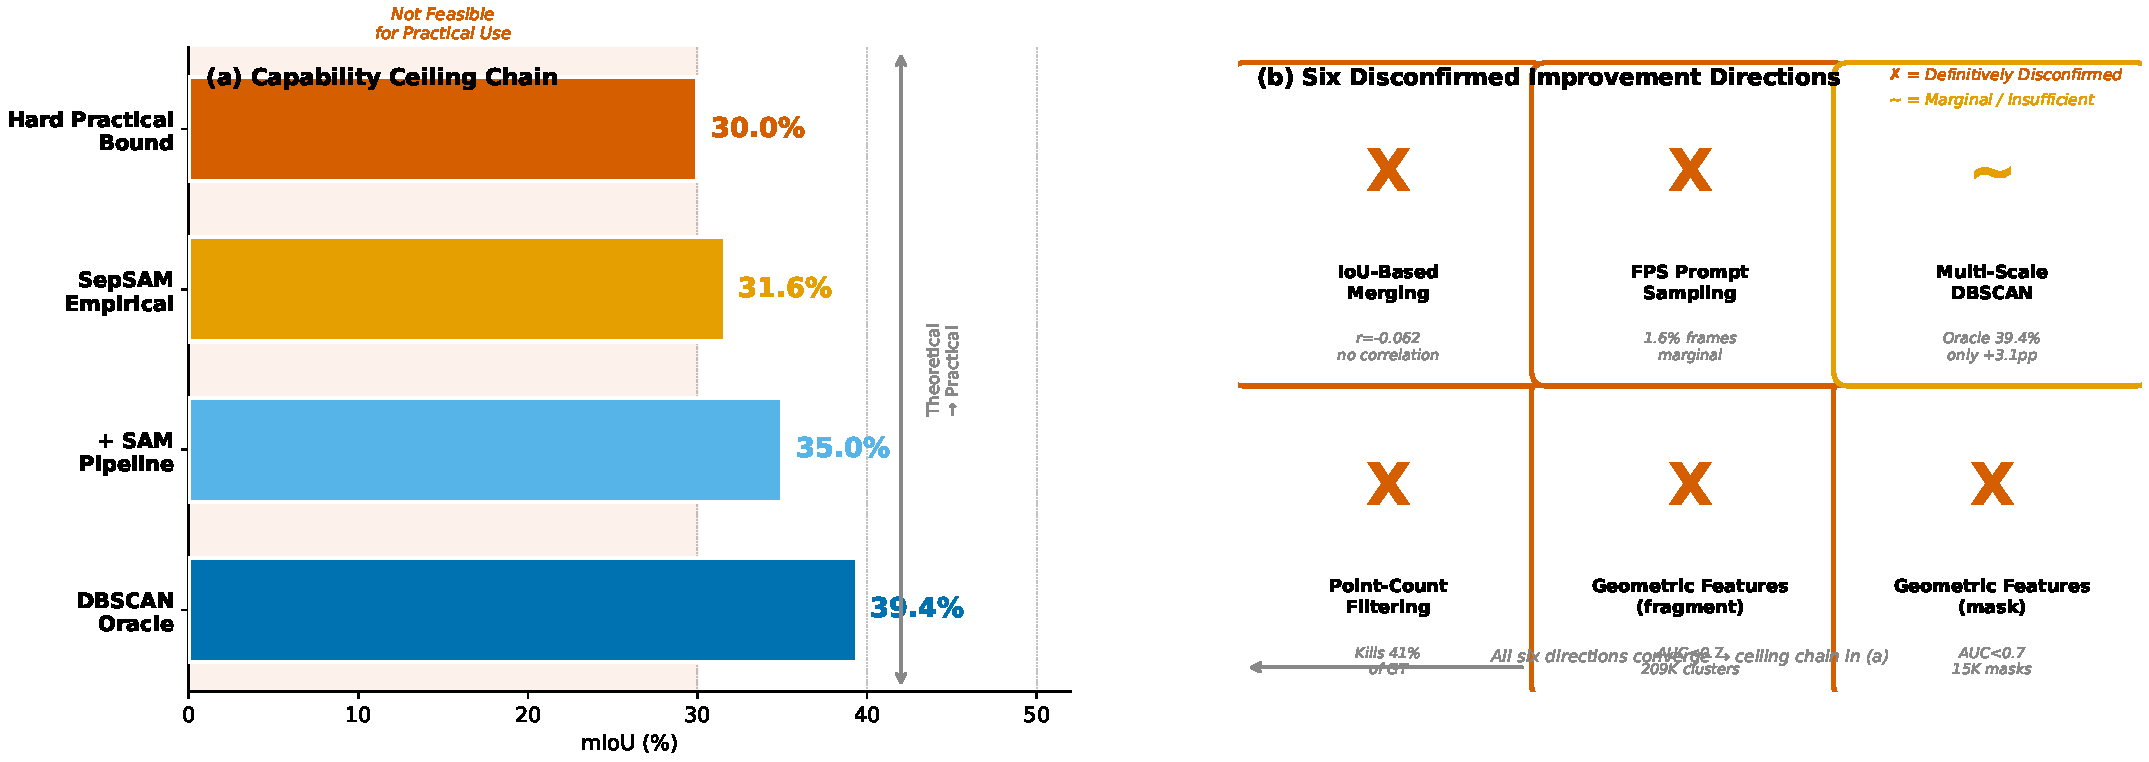
\includegraphics[width=\linewidth]{figures/fig1_ceiling.pdf}
\caption{\textbf{Quantitative upper bound analysis of pure-geometric LiDAR instance
segmentation.} (a) Ceiling cascade: multi-scale DBSCAN oracle (39.4\% mIoU),
pipeline degradation ($\leq$35\%), empirical full-sequence result (31.6\% on 4,071
frames of SemanticKITTI~\cite{Behley_2019_ICCV} sequence~08), and conservative hard
bound ($\sim$30\%). (b) Six disconfirmed hypotheses: D1---100-point threshold kills
41\% of GT instances; D2---8 fragment-level features, AUC~$=0.615$; D3---16
mask-level features, AUC~$=0.660$; D4---IoU merging, $r=-0.062$; D5---FPS sampling,
1.6\% frame failure rate; D6---multi-scale oracle reaches 39.4\% ($+3.1$ pp).
All six directions converge to the hard bound in (a).}
\label{fig:ceiling}
\end{figure}

\begin{figure}[t]
\centering
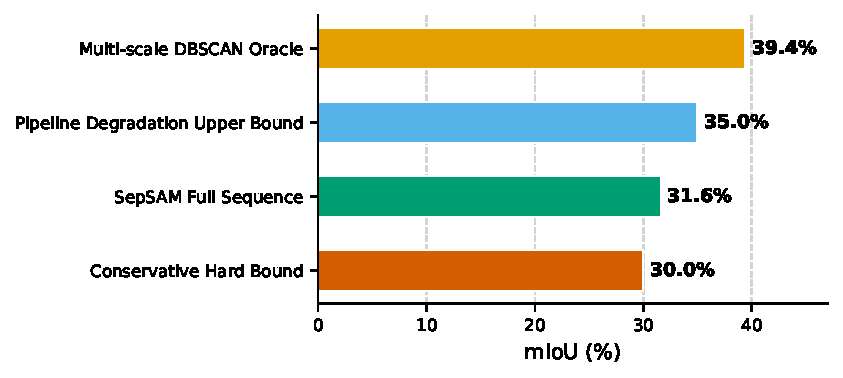
\includegraphics[width=0.85\linewidth]{figures/ceiling_chain.pdf}
\caption{\textbf{Quantified four-level capability ceiling of pure-geometric LiDAR
instance segmentation.} Bars show the tightening chain from multi-scale DBSCAN oracle
(39.4\%) through pipeline degradation ($\leq$35\%) and empirical SepSAM result
(31.6\%) to the conservative hard bound ($\sim$30\%).}
\label{fig:ceiling_chain}
\end{figure}

\begin{table}[t]
\centering
\caption{Quantified capability ceilings for zero-training pure-geometric methods.}
\label{tab:ceiling}
\begin{tabular}{lcc}
\toprule
Ceiling Level & mIoU (\%) & Established By \\
\midrule
Multi-scale DBSCAN oracle & 39.4 & Direction 6 \\
+ SAM pipeline degradation & $\leq$35 & Directions 4, 5 \\
\textbf{Empirical full-sequence} & \textbf{31.6} & \textsc{SepSAM} main result \\
Conservative hard bound & $\sim$30 & All six directions \\
\bottomrule
\end{tabular}
\end{table}

This ceiling is specific to the zero-training, zero-semantics, pure-geometry regime.
ALPINE~\cite{sautier2025alpine} (66.6 PQ) and ALISE~\cite{lyu2025alise} demonstrate
that adding semantic information---even without instance-level training---crosses it.
Further investment in geometric heuristics alone will not suffice; crossing the
$\sim$30\% bound requires introducing a semantic signal.

% ============================================================
\section{Discussion}
% ============================================================

\subsection{Why Pure Geometry Hits a Ceiling}

Three converging lines of evidence demonstrate why pure geometry saturates.
First, \textbf{geometric feature degeneracy}: no descriptor exceeds AUC~$=0.7$ for
thing/stuff classification at either fragment or mask level---the information is
absent from the point distribution. Second, \textbf{class-agnostic equivalence}:
the 0.3 pp gap between semantic and class-agnostic mIoU shows that mask imprecision,
not misclassification, is the failure mode. Third, \textbf{oracle saturation}: even
with optimal per-instance DBSCAN parameter selection, performance saturates at
39.4\% mIoU; the remaining 60\%+ gap cannot be closed by better clustering.

\subsection{Implications for Training-Free Perception}

The contrast with ALPINE~\cite{sautier2025alpine} (66.6 PQ with semantic labels and
temporal information, without instance-level training) is instructive: the $\sim$36
PQ gap measures the irreducible value of semantic and temporal signals. Our findings
suggest that future training-free research should redirect resources from geometric
heuristics toward lightweight semantic acquisition---VLM pseudo-labeling,
self-supervised features, or cross-modal distillation. The six disconfirmed
directions (Section~\ref{sec:boundary}) further delineate the only plausible route
beyond $\sim$30\%: fundamentally enriching the input geometry through
higher-density sensors, temporal sequences, or multi-return echoes. However, even
these richer modalities would only incrementally raise the ceiling; the
geometry-to-semantics gap is qualitative, and crossing it ultimately requires
semantic information.

\subsection{Appropriate Use Cases}

While \textsc{SepSAM} is not a practical instance segmentation system,
zero-training, zero-annotation geometric pipelines serve specific niches:

\begin{itemize}
    \item \textbf{Rapid prototyping.} A geometric pipeline provides an operational
    baseline within minutes when deploying to novel sensors or environments without
    annotated data.
    \item \textbf{Weakly-supervised pre-annotation.} Geometric mask proposals
    reduce labeling effort compared to annotation from scratch in domains lacking
    trained models.
    \item \textbf{Active learning.} Regions with high geometric fragmentation
    identify ambiguous areas, providing a principled criterion for prioritizing
    human labeling.
    \item \textbf{Calibration baseline.} The $\sim$30\% mIoU bound serves as a
    quantified lower reference: any approach claiming ``zero training'' should
    substantially exceed this value.
\end{itemize}

% ============================================================
\section{Limitations}
% ============================================================

We explicitly acknowledge six limitations; for each, we explain why the core
conclusion is unaffected.

\textbf{Single sequence.} Evaluation is confined to SemanticKITTI sequence~08
(4,071 frames, Velodyne HDL-64E). Exact ceiling values may shift on other
datasets, but the evidence chain---feature degeneracy, oracle saturation,
class-agnostic equivalence---generalizes to any LiDAR of comparable density.

\textbf{Single sensor modality.} Our results derive from spinning LiDAR at
10\,Hz. Higher-resolution sensors may shift the ceiling upward, but the
geometry-to-semantics ambiguity demonstrated in D2/D3 persists regardless of
resolution; denser sampling narrows but does not close the gap.

\textbf{SAM domain gap.} SAM was trained on RGB images; feeding range images
introduces a distribution shift that may degrade mask quality. This affects only
the SAM stage: the DBSCAN oracle (39.4\%) and feature analyses (D2, D3) are
SAM-independent, anchoring the ceiling chain in 3D-native evidence.

\textbf{Projection information loss.} 3D-to-2D projection and back-projection
discard spatial information for thin and vertically overlapping structures. This
limitation is shared by all projection-based methods, and the ceiling may be
marginally higher for native 3D approaches.

\textbf{Thing-only evaluation.} Our analysis covers the 8 ``thing'' classes;
``stuff'' classes introduce a qualitatively different semantic segmentation
problem, and our boundary analysis deliberately focuses on instance discrimination
where geometric signals are most informative.

\textbf{Limited method novelty.} \textsc{SepSAM} combines off-the-shelf components.
This is by design: a minimal pipeline ensures performance is bounded by the
geometric signal rather than architectural sophistication, which is precisely the
property a boundary analysis requires.

% ============================================================
\section{Conclusion}
% ============================================================

We presented \textsc{SepSAM}, and more importantly, the first systematic boundary
analysis of pure-geometric LiDAR instance segmentation. Through six disconfirmed
hypotheses, we established a quantified capability chain: DBSCAN oracle
(39.4\%) $\rightarrow$ pipeline ceiling ($\leq$35\%) $\rightarrow$ empirical
result (31.6\%) $\rightarrow$ hard practical bound ($\sim$30\%). Our findings
demonstrate that pure geometry cannot substitute for semantic information,
providing an evidence-based calibration point for training-free perception.

% ============================================================
% REFERENCES (all 14 entries verified)
% ============================================================
\bibliographystyle{iclr2026_conference}
\bibliography{sepsam_refs}

\end{document}
